\documentclass[a4paper]{article}
\usepackage[utf8x]{inputenc}
\usepackage[T1,T2A]{fontenc}
\usepackage[russian]{babel}
\usepackage{hyperref}
\usepackage{indentfirst}
\usepackage{listings}
\usepackage{color}
\usepackage{here}
\usepackage{array}
\usepackage{multirow}
\usepackage{graphicx}
\usepackage[space]{grffile}

\usepackage{caption}
\renewcommand{\lstlistingname}{Программа} % заголовок листингов кода

\usepackage{listings}
\lstset{ %
extendedchars=\true,
keepspaces=true,
language=bash,					% choose the language of the code
basicstyle=\footnotesize,		% the size of the fonts that are used for the code
numbers=left,					% where to put the line-numbers
numberstyle=\footnotesize,		% the size of the fonts that are used for the line-numbers
stepnumber=1,					% the step between two line-numbers. If it is 1 each line will be numbered
numbersep=5pt,					% how far the line-numbers are from the code
backgroundcolor=\color{white},	% choose the background color. You must add \usepackage{color}
showspaces=false				% show spaces adding particular underscores
showstringspaces=false,			% underline spaces within strings
showtabs=false,					% show tabs within strings adding particular underscores
frame=single,           		% adds a frame around the code
tabsize=2,						% sets default tabsize to 2 spaces
captionpos=b,					% sets the caption-position to bottom
breaklines=true,				% sets automatic line breaking
breakatwhitespace=false,		% sets if automatic breaks should only happen at whitespace
escapeinside={\%*}{*)},			% if you want to add a comment within your code
postbreak=\raisebox{0ex}[0ex][0ex]{\ensuremath{\color{red}\hookrightarrow\space}}
}

\usepackage[left=2cm,right=2cm,
top=2cm,bottom=2cm,bindingoffset=0cm]{geometry}



\begin{document}	% начало документа

\begin{titlepage}	% начало титульной страницы

	\begin{center}		% выравнивание по центру

		\large Санкт-Петербургский Политехнический Университет Петра Великого\\
		\large Институт компьютерных наук и технологий \\
		\large Кафедра компьютерных систем и программных технологий\\[6cm]
		% название института, затем отступ 6см
		
		\huge Методы и средства защиты информации\\[0.5cm] % название работы, затем отступ 0,5см
		\large Отчет по лабораторной работе №2\\[0.1cm]
		\large Утилита для исследования сети и сканер портов Nmap\\[5cm]

	\end{center}


	\begin{flushright} % выравнивание по правому краю
		\begin{minipage}{0.25\textwidth} % врезка в половину ширины текста
			\begin{flushleft} % выровнять её содержимое по левому краю

				\large\textbf{Работу выполнил:}\\
				\large Косолапов С.А.\\
				\large {Группа:} 53501/3\\
				
				\large \textbf{Преподаватель:}\\
				\large Вылегжанина К.Д.

			\end{flushleft}
		\end{minipage}
	\end{flushright}
	
	\vfill % заполнить всё доступное ниже пространство

	\begin{center}
	\large Санкт-Петербург\\
	\large \the\year % вывести дату
	\end{center} % закончить выравнивание по центру

\thispagestyle{empty} % не нумеровать страницу
\end{titlepage} % конец титульной страницы

\vfill % заполнить всё доступное ниже пространство


% Содержание
\tableofcontents
\newpage



\section{Цель работы}

Изучить способы и особенности применения утилиты nmap. Определить набор и версии сервисов запущенных на компьютере в диапазоне адресов

\section{Программа работы}

\begin{enumerate}

\item Провести поиск активных хостов

\item Определить открытые порты

\item Определить версии сервисов

\item Изучить файлы nmap-services, nmap-os-db, nmap-service-probes

\item Добавить новую сигнатуру службы в файл nmap-service-probes (для этого создать минимальный tcp server, добиться, чтобы при сканировании nmap указывал для него название и версию)

\item Сохранить вывод утилиты в формате xml

\item Исследовать различные этапы и режимы работы nmap с использованием утилиты Wireshark

\end{enumerate}

Просканировать виртуальную машину Metasploitable2 используя db\_nmap из состава metasploit-framework

Выбрать пять записей из файла nmap-service-probes и описать их работу Выбрать один скрипт из состава Nmap и описать его работу

\section{Теоретическая информация}

Утилита nmap является утилитой с открытым исходным кодом, позволяющей производить сканирование сети и обнаруживать уязвимости в исследуемых узлах (открытые порты). Данная утилита использует "сырые" IP-пакеты нестандартными способами для обнаружения хостов в сети, а так же установленных на них операционных систем, типы пакетных фильтров и брандмауэров, используемые службы и так далее.

\section{Ход выполнения работы}

В работе используются две сконфигурированные виртуальные машины - Kali Linux 1.0.6 (последняя версия, увы, не заработала в супервизоре) и metasploitable2 в качестве машины для сканирования и поведения атак с ip-адресами 10.0.0.1 и 10.0.0.2 соответственно.

Установка привязка адресов к интерфейсам и проверка производились следующим образом:

\lstinputlisting[numbers=none, keywords={}]{log/network-establish.txt}

\subsection{Провести поиск активных хостов}

В новых версиях nmap это делается с опцией -sn. В предыдущих версиях Nmap опция -sn выглядит, как -sP. 

Вот некоторые другие варианты сканирования:

\begin{itemize}
\item -sL - вырожденное сканирование всех подряд хостов, без посылки пакетов хостам
\item -sn | -sP - пинг-сканирование
\item -Pn - не использовать пинг-сканирование
\item -PS <list of ports> - TCP SYN сканирование. Позволяет определить, открыт ли порт (в зависимости от ответа на посланный SYN).
\item -PA <list of ports> - TCP ACK сканирование. Позволяет определить существование порта. В ответ прослушиваемый порт будет отдавать RST.
\item ...
\item -n не производить разрешение DNS имён
\item --traceroute - отслеживать путь
\end{itemize}

\lstinputlisting[numbers=none, keywords={}]{log/active-hosts.txt}

Таким образом, видим, что nmap обнаружил имеющийся хост.

\subsection{Определить открытые порты}

Такую операцию выполняет утилита без опций, либо можно указать, например, опции -PS или -PA.

\lstinputlisting[numbers=none, keywords={}, lastline=32]{log/active-ports.txt}

\lstinputlisting[numbers=none, keywords={}, firstline=65]{log/active-ports.txt}

Результаты в целом совпадают, однако, по непонятным причинам, в первом случае 53 DNS-порт оказался закрыт, а во втором он открылся. При повторе эксперимента с -PS порт указан, как открытый.

\subsection{Определить версии сервисов}

Это можно сделать с помощью опции -sV.

Результат определения версий:

\lstinputlisting[numbers=none, keywords={}, keywords={}]{log/versions.txt}

Судя по всему, из-за более старой версии nmap, чем metasploitable2, nmap не сумел определить приложение на порте 8180. На этом порте располагается сервис Apache Tomcat.

\subsection{Изучить файлы nmap-services, nmap-os-db, nmap-service-probes}

Эти файлы являются служебными и располагаются в директории /usr/share/nmap.

\lstinputlisting[language=bash, lastline=14]{log/service-files.txt}

\subsubsection{Файл nmap-services}

Файл содержит описание привязки портов и протоколов к сервисам.

\lstinputlisting[numbers=none, keywords={}, firstline=15, lastline=108]{log/service-files.txt}

Как видим, каждая строка файла описана в следующем формате:

\begin{lstlisting}
service-name port/protocol
\end{lstlisting}

Как видим, для большинства сервисов определены различные протоколы и порты. 

\subsubsection{Файл nmap\-os\-db}

Nmap позволяет определить сигнатуры (отпечатки, fingerprints) ответов на запросы к различным протоколам и портам, за счёт чего и производится определение ОС атакуемого. Дело в том, что различные ОС по-разному реализуют многие аспекты таких протоколов, как TCP, UDP, ICMP и т.д. Исходя из того, что, в зависимости от ОС, поля могут быть по-разному заполнены, а время ответа может варьироваться, можно с большой вероятностью установить, какая это операционная система. Правда nmap в случае, если не может по отпечаткам точно идентифицировать систему, не использует вероятностный подход, а пишет, что система не распознана.

Сигнатуры таких параметров как раз и представлены в файле nmap-os-db:

\lstinputlisting[numbers=none, keywords={}, firstline=123, lastline=223]{log/service-files.txt}

Проверить ОС атакуемого можно следующим образом:

\lstinputlisting[numbers=none, keywords={}]{log/os-detection.txt}

Первый эксперимент показывает, что при запрете сканирования портов нет никакой возможности установить тип и версию ОС. Дальнейший эксперимент показывает, что metasploitable2 построена на ядре Linux 2.6.x. Знание типа и версии ОС является одним из фундаментов для построения атаки.

\subsubsection{Файл nmap-service-probes}

При сканировании, в первую очередь, nmap полагается на информацию, описанную в файле nmap-services, где описано стандартное использование портов. Вместе с тем, вполне возможно, что назначение стандартного порта было переопределено, что, казалось бы, может добавить сложности при проведении атаки. Однако nmap анализирует также и отклик служб на описанные запросы. Как раз такие описания и содержит в себе файл nmap\-service\-probes. Вот некоторые директивы, которые можно описать в этом файле:

\begin{itemize}

\item probe
\begin{verbatim}
Probe <protocol> <probename> <probestring>
\end{verbatim}

Описывает строку, которую nmap будет посылать атакуемому серверу.

\item match
\begin{verbatim}
match <service> <pattern> [<versioninfo>]
\end{verbatim}

Позволяет описать, как распознать ответ атакуемого сервера на посылку, описанную в probe, на основе чего можно сделать заключение о том, что это за сервис и его версии.

\item ports и sslports
\begin{verbatim}
ports <portlist>
\end{verbatim}

Позволяет определить, какие порты обычно обнаруживаются. Строка ports/sslports должна быть одна на каждую probe-секцию.

\item exclude
\begin{verbatim}
Exclude <port specification>
\end{verbatim}

Директива исключает порты из сканирования версий.

\end{itemize}

\lstinputlisting[numbers=none, keywords={}, firstline=225]{log/service-files.txt}

\subsection{Добавить новую сигнатуру службы в файл nmap-service-probes (для этого создать минимальный tcp server, добиться, чтобы при сканировании nmap указывал для него название и версию)}

Для исследования использовался простейший сервер:

\lstinputlisting[language=c, caption=Код сервера]{code/server.c}

Для того, чтобы сервис определился, необходимо прописать в файле nmap-service-probes информацию, позволяющую его идентифицировать. В регулярном выражении в директиве match необходимо специфицировать ответ сервера, в котором можно выделить версию.

\lstinputlisting[lastline=6]{log/server.txt}

В результате, можем идентифицировать работающий на сканируемой машине сервер:

\lstinputlisting[language=bash, firstline=10]{log/server.txt}

\subsection{Сохранить вывод утилиты в формате xml}

Вывод в xml осуществляется с помощью опции -X, в сочетании с которой можно вывести в файл. Ниже представлен пример вызова nmap с сохранением в xml.

\lstinputlisting[numbers=none, keywords={}]{log/xmlscan.txt}

Вывод будет осуществлён в файл output.xml:

\lstinputlisting[language=xml, caption=Выходной xml-файл]{log/output.xml}

\subsection{Исследовать различные этапы и режимы работы nmap с использованием утилиты Wireshark}

При анализе metasploitable2 с помощью nmap без параметров (кроме адреса) суммарно уходят и приходят порядка 2000 пакетов. 

Изначально для сервисов на сканируемой машине посылаются TCP SYN-запросы. Они составляют подавляющее количество исходящих пакетов. Также среди исходящих встречаются TCP RST-пакеты - для тех сервисов, которые ответили на SYN-запросы. Таких посылок 23. Однако определённых сервисов - 22. Таким образом, один сервис, судя по всему, не проходит дополнительную фильтрацию.

\begin{figure}[H]
	\begin{center}
		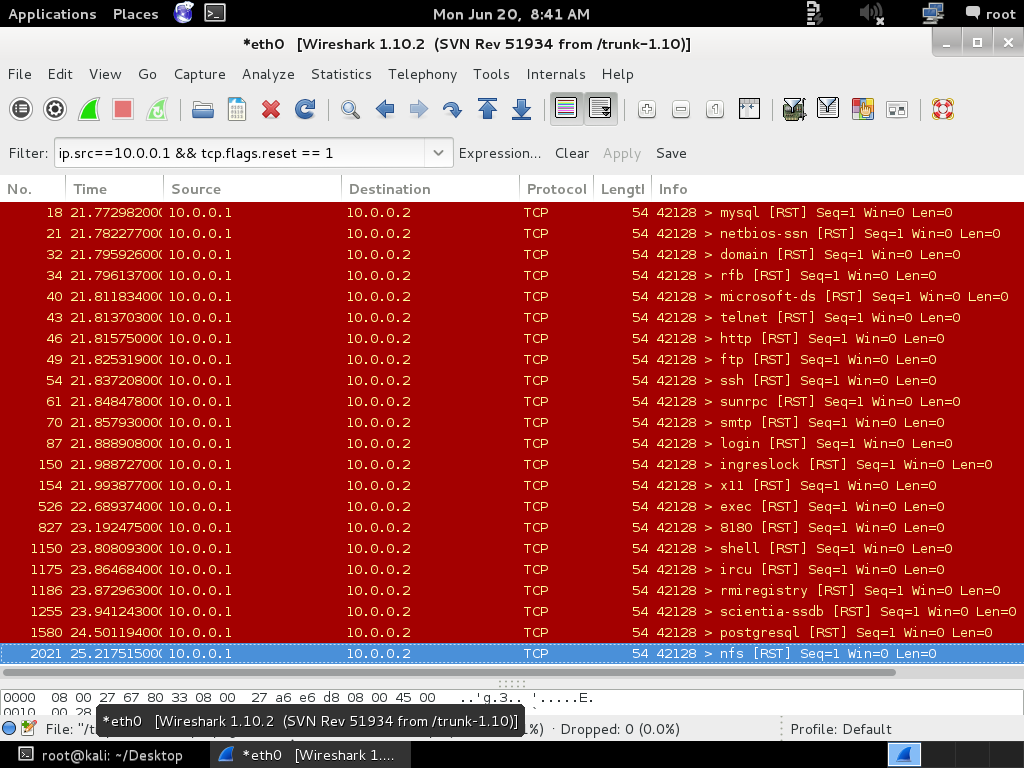
\includegraphics[scale=0.5]{pics/rst_wireshark.png}
		\caption{Демонстрация исходящих RST-пакетов} 
		\label{pic:pic_name}
	\end{center}
\end{figure}

В случае, если всё хорошо и порт прослушивается, в ответ приходит пакет с флагами (SYN, ACK), в ответ на который посылается RST:

\begin{figure}[H]
	\begin{center}
		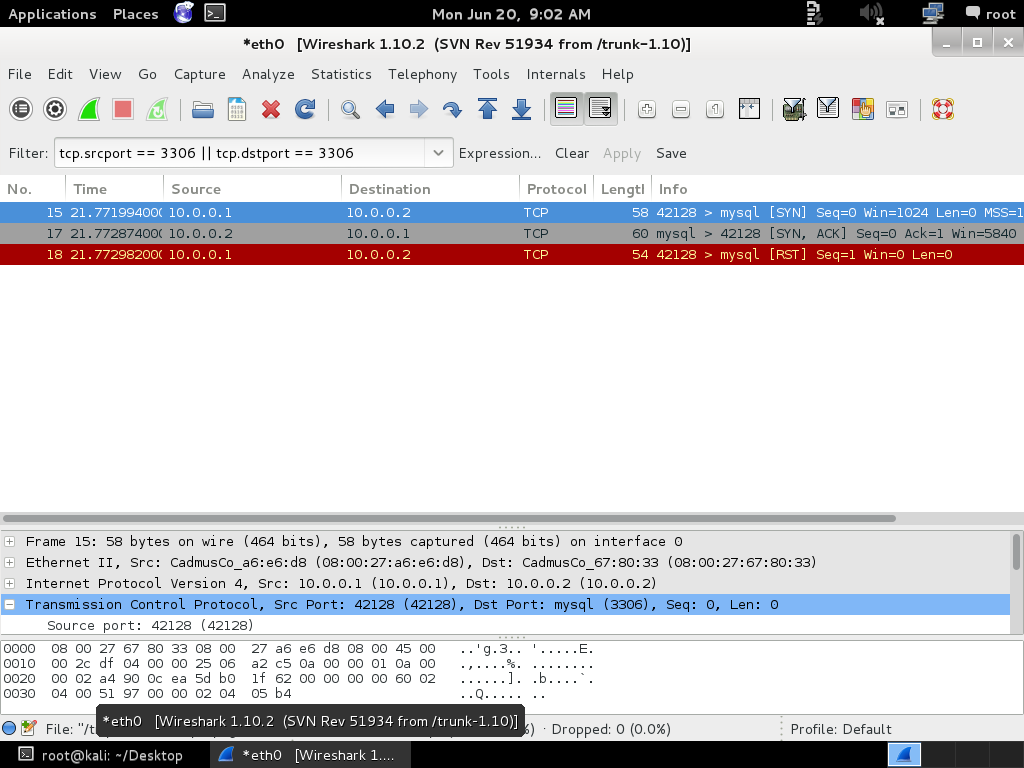
\includegraphics[scale=0.5]{pics/good_tcp.png}
		\caption{Демонстрация определения прослушиваемого порта} 
		\label{pic:pic_name}
	\end{center}
\end{figure}

В случае же, если порт не прослушивается сервисами на стороне сканируемой машины, в ответ приходит пакет с флагами (RST, ACK).

\begin{figure}[H]
	\begin{center}
		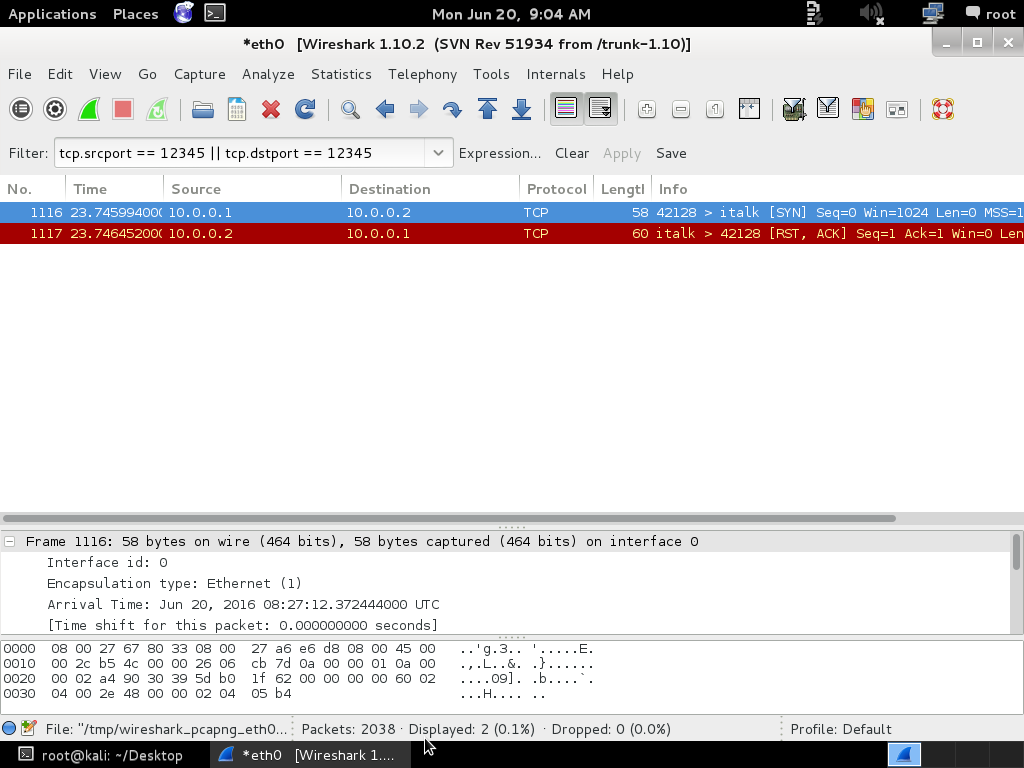
\includegraphics[scale=0.5]{pics/bad_tcp.png}
		\caption{Демонстрация определения непрослушиваемого порта} 
		\label{pic:pic_name}
	\end{center}
\end{figure}

\subsection{Просканировать виртуальную машину Metasploitable2 используя db\_nmap из состава metasploit-framework}

Начальным этапом служит настройка фреймворка. До Kali2.0 использовался Metasploit вместо metasploit framework, и детали настройки несколько отличаются. В частности, отсутствует утилита msfdb, с помощью которой производится инициализация базы данных в последующих релизах. Инициализация производится при старте msfconsole.

\lstinputlisting[numbers=none, keywords={}, lastline=32]{log/db.txt}

Далее можно сделать сканирование с помощью nmap, но уже внутри msfconsole. В данном случае результат совпадает с представленным выше.

\lstinputlisting[numbers=none, keywords={}, firstline=33]{log/db.txt}

\subsection{Выбрать один скрипт из состава Nmap и описать его работу}

Nmap поддерживает скрипты, описанные на языке Lua (в рамках NSE - nmap scripting engine). Найти скрипты можно по адресу: https://nmap.org/nsedoc/.

Был взят один из размещённых там скриптов.

Главной функцией в скриптах является функция action(host, port). Перед ней следуют блоки description, присваиваются значения переменным author, license, categories (категории, к которым можно определить скрипт). Ниже представлен вариант скрипта, реализующий вывод информации о формате amqp, используемого в RabbitMQ.

\lstinputlisting[language={[5.0]Lua}]{code/amqp-info.nse}

Этот скрипт позволяет подготовиться к атаке при использовании amqp. Создаётся клиент, устанавливается соединение, извлекаются параметры (имя, название продукта и т.д.). Затем полученные параметры записываются  в объект port, переданный в функцию.

\subsection{Выбрать пять записей из файла nmap-service-probes и описать их работу}

\begin{enumerate}

\item
\begin{lstlisting}[numbers=none, keywords={}]
match asterisk m|^Asterisk Call Manager/([\d.]+)\r\n| p/Asterisk Call Manager/ v/$1/ cpe: a:digium:asterisk:$1/
\end{lstlisting}

Сначала должно быть описание приложения - ""Asterisk Call Manager"", затем ищет числа, разделённые точкой.  Далее указано выводимое описание - название продукта (p), версия (v), которая парсится описанным ранее регулярным выражением, далее идёт описание CPE (стандартный формат наименования программных продуктов).

\item
\begin{lstlisting}[numbers=none, keywords={}]
Exclude T:9100-9107
\end{lstlisting}

Исключить порты с 9100 по 9107.

\item
\begin{lstlisting}[numbers=none, keywords={}]
Probe TCP NULL q||
\end{lstlisting}

Задаётся имя и формат посылки. В данном случае - для TCP, имя NULL, далее описывается посылаемое сообщение  - в данном случае оно пустое. Т.е. далее в директивах match описываются сигнатуры реакций сервисов на данный запрос.

\item
\begin{lstlisting}[numbers=none, keywords={}]
match someServer m/^Greeting \((\w*) ([\d.]*)\)/ p/$1/ v/$2/
\end{lstlisting}

Описывается представленный выше сервер. Сначала ожидается слово Greeting, далее в скобках - сначала слово, а затем версия, заданные регулярными выражениями. Далее описывается имя продукта - слово, распарсенное из первого регулярного выражения, а затем версия продукта - число из второго регулярного выражения.

\item
\begin{lstlisting}[numbers=none, keywords={}]
match asterisk-proxy m|^Response: Follows\r\nPrivilege: Command\r\n--END COMMAND--\r\n| p/Asterisk Call Manager Proxy/ cpe:/a:digium:asterisk/ 
\end{lstlisting}

В ответе должна содержаться строка, указанная между \textasciicircum  и CPE. Далее описывается CPE.

\end{enumerate}

\section{Выводы}

В работе рассмотрена утилита nmap. Она позволяет сканировать удалённые хосты на наличие открытых портов, а следовательно, искать уязвимости в них. С её помощью можно определить наименование и версию операционной системы, названия и версии используемых сервисов, привязанных к определённых портам. Можно произвести анализ соответствия сервиса, привязанного к определённому порту, стандартному назначению порта. Также можно редактировать и добавлять свои сигнатуры в файлы, используемые утилитой nmap, тонко настраивать порты сканирования и параметры отображения. Утилита входит в состав пакетов Metasploit и Fetasploit Framework. Также утилита nmap имеет свой скриптовой движок и позволяет использовать готовые или писать свои скрипты. Nmap является одним из фундаментов при подготовке и проведении атаки на удалённый хост.

\end{document}